% 
% Annual Cognitive Science Conference
% Sample LaTeX Paper -- Proceedings Format
% \


% to do
% -- consistent names of conditions: listener uncertainty in common ground vs. not
% -----

\documentclass[10pt,letterpaper]{article}

\usepackage{cogsci}
\usepackage{pslatex}
\usepackage{apacite}
\usepackage{url}
\usepackage{graphicx}
\usepackage{caption}
\usepackage{subcaption}
\usepackage{listings}
\usepackage{color}
\usepackage{textcomp}
\usepackage{amsmath}
\usepackage{amssymb}
\usepackage{wrapfig}
\usepackage{lipsum}
\usepackage{epigraph}

\graphicspath{{figures/}}

\def\signed #1{{\leavevmode\unskip\nobreak\hfil\penalty50\hskip2em
  \hbox{}\nobreak\hfil(#1)%
  \parfillskip=0pt \finalhyphendemerits=0 \endgraf}}

\newsavebox\mybox
\newenvironment{aquote}[1]
  {\savebox\mybox{#1}\begin{quote}}
  {\signed{\usebox\mybox}\end{quote}}

 \newcommand{\denote}[1]{\mbox{ $[\![ #1 ]\!]$}}

\definecolor{Red}{RGB}{255,0,0}
\newcommand{\red}[1]{\textcolor{Red}{#1}}  

\definecolor{Blue}{RGB}{0,0,255}
\newcommand{\blue}[1]{\textcolor{Blue}{#1}}  
\definecolor{Green}{RGB}{10,200,100}
\newcommand{\ndg}[1]{\textcolor{Green}{[ndg: #1]}}  
\newcommand{\mht}[1]{\textcolor{Blue}{[mht: #1]}}  


\title{It goes without saying: When an assertion is evidence against itself}

\definecolor{DarkOrange}{RGB}{255,100,50}
\newcommand{\ellen}[1]{\textcolor{DarkOrange}{[ellen: #1]}}  

%\title{It goes without saying: The pragmatics of uninformative utterances}

\author{ {\large \bf Michael Henry Tessler*}, {\large \bf Eleanor K. Chestnut*},
{\large \bf Ellen M. Markman}, and {\large \bf Noah D. Goodman}  \\
\{mtessler, ekc, markman, ngoodman\} @stanford.edu \\ 
  Department of Psychology, Stanford University \\
  *Authors contributed equally to this work.}

\begin{document}

\maketitle


\begin{abstract}
%\ndg{abstract is too technical. start with the puzzle of how asserting a proposition can sometimes decrease its plausibility. the use of common ground here is kind of hard to follow.}
If you just met Jane and her friend tells you, ``Jane went on a hike today", you might think Jane is the kind of person who likes to go on hikes.  
However, ``Jane wore shoes today'' seems to imply the opposite. 
In this case, listeners infer that Jane does \emph{not} like to wear shoes (e.g., \cite{Kravtchenko2015}.  
Why should some utterances serve as evidence for a given habit, while others 'backfire' and serve as evidence against it?  
We present a formal model of language understanding that can revise information that is common ground when an utterance is uninformative with respect to prior beliefs.  
The model predicts that this ``backfiring'' inference relies on shared knowledge between speaker and listener, which we manipulate in Experiment 1, and \emph{a priori} beliefs about the event under discussion, which we manipulate and measure in Experiment 2. 
%In Experiment 1, we show that this inference does not occur when interlocutors are mutually aware of information in common ground, or when a statement is removed from a conversational context.  In Experiment 2, we show that the \emph{existence} and \emph{strength} of this inference depends on the listener's prior  beliefs., which we measure empirically.
% Finally, we present a computational model that predicts these results.
% that when an utterance is redundant with the prior beliefs of the listener (most people wear shoes and shoe-wearing tends to happen everyday), adults will revise information that is in common ground with the speaker (here, that Jane typically wears shoes) so that the utterance becomes informative.  
%Successful communication requires a mutually understood set of beliefs between speaker and listener.
%When common ground is not shared, a listener can use a speaker's utterance in conjunction with conversational principles to infer what was assumed by the speaker.
%Previous work has shown that this inference can have surprising ramifications, including decreasing the belief in the proposition that was asserted by the speaker 
%(e.g. upon hearing, ``John paid the cashier!'', listeners infer that John does not typically pay for his groceries).
% i just think we need an example somewhere in here
%Here, we formalize inferences about common ground using the case when a speaker's utterance refers to something that should already be in common ground.
%The formal pragmatics model makes clear that this kind of utterance will backfire (i.e. imply that the opposite is typically true) when the interlocutors do not share common ground, but not when they do.
% the last sentence is a little hard to read because of many "not"s... but we can worry about that later.
%Language is interpreted in context with respect to some common ground between speaker and listener.
%Common ground can make certain utterances uninformative (e.g. stating something obvious), but is plausibly revised in the face of uninformative utterances.
%In Expt.~1, we verify this prediction using a paradigm that makes the 

\textbf{Keywords:} 
pragmatics; language; common ground; Bayesian model
\end{abstract}


%\begin{quotation}
%\small
%``I am not a crook.'' -- Richard Nixon

%\end{quotation}

%In one of the most infamous moments in U.S. presidential history, Richard Nixon declared to the press corps, "I am not a crook"€ (CITE).  On the surface, this claim argues for Nixon's innocence, as it literally states that he is not a crook.  As several researchers have shown, however, this statement contains a number of pragmatic implications that actually counter its literal, semantic meaning (CITE).  Nixon'€™s claim, for instance, presupposes that others believed that he was a crook; otherwise, it would not have been an informative statement to make, since most people presumably are not crooks (Grice, 1975).  Thus, if a listener is not aware of the Watergate scandal, or if they have no reason to question Nixon's moral status, they might actually learn from this claim that Nixon was likely corrupt in some way.

In 1973, beleaguered U.S. President Richard Nixon declared to the press corps, ``I am not a crook'' \cite{NixonQuote}.  
If we were to take Nixon's words at face value, they would seem to suggest that he is a good guy, since that is what the words literally mean.
However, the fact that Nixon said this, which---for a president, at least---should go without saying, we take his utterance to imply that he is actually somehow corrupt.

%% I'd like to avoid technical words (literal, pragmatic) and citations in the first few sentences... Should be something a non-language person can appreciate
%On a literal level, this claim argues for Nixon's innocence.  
%Pragmatically, however, this claim presupposes that someone has accused Nixon of a crime; otherwise, the claim would not be informative (Grice, 1975).  
%Thus, contrary to Nixon's intentions, a listener unaware of the Watergate scandal could actually \emph{learn} from this utterance that Nixon was associated with corruption.

To date, this phenomenon---that utterances can ``backfire" (i.e., decrease a listener's belief in the content being asserted)---is not well understood.  Instead, the standard Bayesian treatment of learning from testimony has stressed that we update our beliefs about the world to be  \emph{in accordance} with information expressed through language \red{(cite)}. 
Research in social psychology, however, has shown that a headline such as ``Robert Kennedy was not planning the assassination of Fidel Castro" causes adults to more strongly believe that Kennedy \emph{had} been planning to assassinate Castro \cite{Wegner1981, Gruenfeld1992, Yandell1979}.
%In the social psychological literature, however, a few studies have found that \emph{a priori} uninformative statements negating negative associations (e.g.,``Bob Talbert not linked with mafia"\footnote{This is uninformative because most people are not in the mafia.})
%cause adults to have a more negative impression of the target (here, Mr. Talbert) than they would otherwise \cite{Wegner1981, Yandell1979}, and can actually cause people to believe the exact opposite of what those lines claim \cite{Gruenfeld1992}.
% A few studies, however, provide evidence that when utterances are redundant with a listener's prior beliefs, they can imply that the opposite of what is expressed. 
% \citeA{Wegner1981}, for example, demonstrated  despite explicitly denying incriminating information. Similarly, Gruenfeld and Wyer (1992) showed that uninformative newspaper lines can actually    
 %\citeA{Gruenfeld1992}, for example, found that fake lines such as ``Robert Kennedy was not planning the assassination of Fidel Castro" caused adults to more strongly believe that Kennedy \emph{had} been planning to assassinate Castro. 
Similarly, \citeA{Kravtchenko2015} recently showed that if a speaker says, ``John paid the cashier!" as part of a story about John's trip to a store, adults infer that John does not typically pay cashiers.

Why do such claims backfire, while others don't? We suggest that this effect depends on the common ground shared between interlocutors, and the conversational principle that utterances should be \emph{cooperative}---that is, both relevant and informative \cite{Grice1975}.  In short, when an utterance does not appear on the surface to be informative, listeners will adjust their understanding of what the speaker believed was in common ground to \emph{make} the utterance informative \red{(CITE)}.

 %in order to \emph{make} the utterance informative (\red{CITE} accommodation?).

In this paper, we formalize a pragmatic language model wherein speaker and listener either do not share common ground about a person's habits (e.g., a student's tendency to turn in her homework on time).  In two experiments, we test three predictions from the model and an alternative model in which common ground is shared: (a) Backfiring should occur when common ground is \emph{not} shared between interlocutors; here, the speaker will be interpreted as presupposing information that the listener was not aware of, thereby causing the listener to infer that information; (b) When common ground \emph{is} shared, standard learning from testimony should occur, because the speaker's utterance will be understood as semantically informative for the listener; and (c) The existence and strength of backfiring should vary according to the strength of the prior beliefs that are redundant with the utterance, since greater redundancy causes utterances to be less informative.



\section{Formalizing backfiring language}


Observing individuals perform an action can be taken as some evidence that they \emph{typically} perform that action, or have the habit $h$ of doing behavior $b$. 
For example, seeing a student turn in her homework provides some evidence that she usually turns in her homework. 
It is a more likely explanation than the alternative (here, that the student does \emph{not} typically turn in her homework).

We formalize this using a simple Bayesian model:
\begin{eqnarray}
P(h \mid b) \propto P(b \mid h) P(h) \label{eq:bayes}
\end{eqnarray}
As a habit is more likely to give rise to the behavior --- as $P(b \mid h)$ gets large --- so too does the behavior become more indicative of the habit, assuming the prior probabilities are constant. 

Knowledge about an event can also come from a helpful speaker.
For example, if a school survey is being conducted, and a principal asks a teacher, ``Did your student turn in her homework today?" then the response, ``Yes, my student turned in her homework today," could be taken as evidence that the student usually turns in her homework.  In this case, the teacher is aware that the principal does not know the habits of his students, so he informs her of them.

%communicating the behavior (here, ``My student turned in his homework today'') can lead the listener to believe the underlying habit (here, that the student \emph{typically} turns in his homework) more strongly.  Critically, in this case, we assume that the person asking, ``Did your student turn in his homework today?" is \emph{not} asking the question because he or she suspects that the habit is absent (i.e., that the student doesn't usually turn in his homework); instead, the person must be asking for an unbiased reason (e.g., perhaps the person is taking a survey of student behavior).  If the person \emph{did} ask the question out of suspicion, then they would clearly already hold the belief that the student does not have the habit, and it is unclear whether the speaker's response would change their opinion.

If, by contrast, a speaker misrepresents the listener's knowledge (e.g., the speaker believes the listener knows something that the listener actually doesn't know, or the listener is overhearing a conversation), communicating the behavior might lead the listener to believe the habit is \emph{less} likely.  If the student did usually turn in her homework, for example, then the utterance---``My student turned in his homework today.'''---would be uninformative.



% it is valid to assume the knowledge of the habit to be communicated is \emph{not} in common ground, but that both teacher and learner have a meta-agreement on this.
%
%\ndg{this paragraph is kind of confusing and doesn't really lead into the formal treatment. revise to emphasize (and show) how to model the three situations in the experiment.}
%In a conversational setting, knowledge of a person's habits may or may not be in common ground, and the speaker and listener may or may not be aware of this \cite{Clark1977, Clark1996}. 

%Friends may also have a mutually-understood common ground about a third person; one that an overhearer might not have. 
%This same situation occurs when one of the friends assumes a bit of knowledge that the other person doesn't have (e.g. because she forgot).
%Other communicative settings may exist, where the both levels of knowledge are not in common ground. 
%If a listener believes that the speaker is not representing her uncertainty correctly (e.g., because the listener has forgotten this bit of information or because the listener is overhearing a conversation), she can use the speech-act to help resolve what the speaker believes to be in common ground. 
%\red{we might still want a concrete example here, but can add it later}

We incorporate these inferences into the Rational Speech-Acts framework \cite{Frank2012, Goodman2013}, as a lifted variable inference akin to the treatment by \citeA{Degen2015} and discussed in detail in \citeA{GoodmanLassiter}\footnote{Briefly, a ``lifted'' variable is a variable of uncertainty over which a pragmatic listener reasons. The inference incorporates general pragmatic principles of communication, by assuming the speaker intended a particular value of that random variable.}.
%
The \textbf{backfiring} RSA model is:  
\begin{eqnarray}
&&P_{L_1}(b, h \mid u)\propto P_{S_1}(u \mid b, h)\cdot P(b \mid h) \cdot P(h) \label{eq:L1}\\
&&P_{S_1}(u \mid b, h) \propto  P_{L_0}(b \mid u, h)^{\alpha} \label{eq:S1}\\
&&P_{L_0}(b \mid u, h)\propto \denote{u}(b) \cdot P(b \mid h) \label{eq:L0}
\end{eqnarray}
%
Here, a pragmatic listener $L_1$ hears an utterance $u$ describing an event or behavior $b$ of a target person and is trying to infer whether that behavior occurred and what are the target's habits $h$ in general. 
The listener assumes this utterance came from a speaker $S_1$, who is knowledgable about the event and about the person's habits. The speaker has the possibility of remarking on the event with an affirmation or a negation --- $b$ or $\neg b$--- as well as the possibility of not remarking on the situation, a \emph{null} utterance that has no information content.  
The speaker reasons about an idealized literal listener $L_0$ in his head. Crucially, the speaker believes the listener to already know about the target person's habits $h$. In this way, the speaker presupposes this habit is in common ground.

The target's behavior can be thought to be distributed in time according to a Poisson distribution:  $b \sim \text{Poisson}(\lambda)$, and the rate $\lambda$  is influenced by whether or not the person has the habit. For now, we assume that if the habit $h$ is present, the behavior occurs with a high rate  $\lambda_{h}$ and if the habit is absent, the rate is lower $\lambda_{\neg h}$,
where $\lambda_{h} > \lambda_{\neg h}$.
In Expt.~2, we relax the notion of discrete habits and consider a continuous distribution over rates. 
The model is implemented in the probabilistic programming language WebPPL \cite{dippl}, and a simple version can be seen at \mht{add forest page}.

\begin{figure}
\centering
    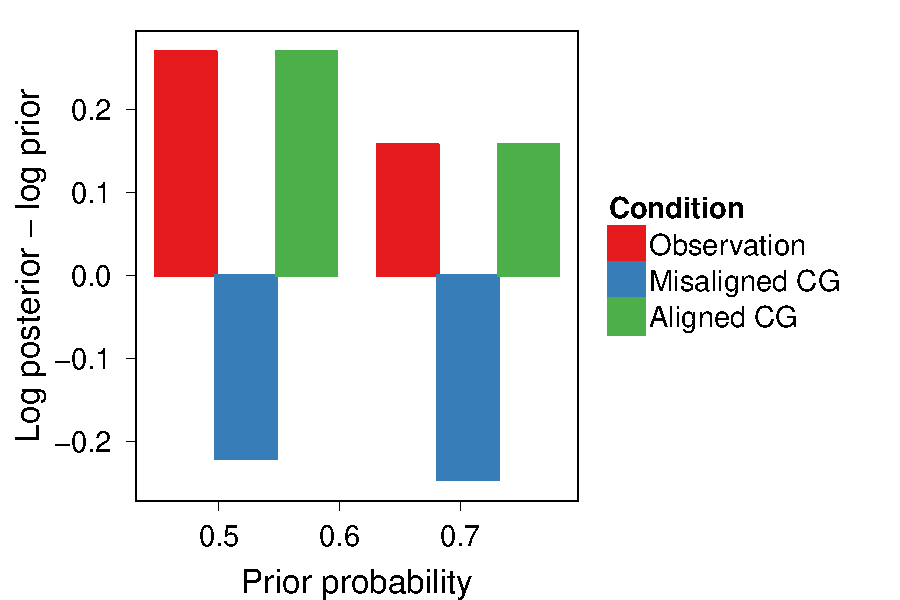
\includegraphics[width=\columnwidth]{schematic-model}
    \caption{Schematic model predictions.
    \mht{Figure to be revised}
    Observing or hearing a proposition when speaker and listener share common ground provides evidence for the underlying habit (green and red bars $> 0$). 
    When common ground is not shared, hearing a proposition provides evidence \emph{against} the underlying habit (blue bars $<0$).
    Additionally, when the prior beliefs about a habit are least informed (prior probability around 0.5), a single observation of the behavior carries a lot of evidence, relative to when prior beliefs are more informed. 
    The opposite is true when words backfire: the stronger the \emph{a priori} belief in the habit, the more the utterance conveys evidence \emph{against} that habit. }
  \label{fig:schematic-model}
\end{figure}


The model's predictions critically rely on the fact that the speaker does not represent the listener's beliefs accurately and are additionally sensitive to the prior probability of the behavior occurring. 
When a habit $h$ is likely to give rise to an event $b$ (i.e., the rate $\lambda$ is sufficiently high), utterances affirming the event will be interpreted as expressing atypical behavior by implicitly implying that the habit is not present ($\neg h$).
The statement, ``My student turned in his homework today,'' for instance, should suggest that the student does \emph{not} usually turn in his homework (Figure \ref{fig:schematic-model} \mht{what would be a good figure to show here?}).
%This occurs when the speaker does not represent the listener's beliefs accurately.
%The strength of this inference is predicted to be modulated the listener's \emph{a priori} belief in the habit; the stronger the listener believes it to be the case that the roommate usually washes her dishes, the more the utterance \emph{My roommate washed her dishes today} will backfire. 

\subsection{Alternative models}

The backfiring inference depends critically on a misunderstanding of common ground. 
If an interlocutor explicitly tells another, for example, ``I need to fill out this report. Did your student turn in his homework today?'' then the speaker will learn that the listener is unsure of the student's habits.
%\footnote{It is also important that the question be asked for plausible reasons that do not imply that the listener believes the habit to be absent (i.e., that the student doesn't usually turn in his homework).}.
As a result, the response, ``My student turned in his homework today,'' will become semantically informative, no longer presupposing that the listener knows about the student's habits.
Figure \ref{fig:schematic-model} (green bars) shows what happens when the speaker and listener are both aware of the listener's knowledge.
This is more akin to pedagogical communication, where teacher and learner are on the same page. 
An \textbf{instructive} RSA model is nearly identical to the one above, with the only difference being the speaker's model of the literal listener:
\begin{eqnarray}
%&&P_{L_1}(b, h \mid u)\propto P_{S_1}(u \mid b)\cdot P(b \mid h) \cdot P(h) \label{eq:L1mod}\\
&&P_{S_1^{*}}(u \mid b) \propto P_{L_0}(b, h \mid u) ^ {\alpha} \label{eq:S1mod}
%&&P_{L_0}(b, h \mid u)\propto \denote{u}(b) \cdot P(b \mid h) \label{eq:L0mod}
\end{eqnarray}
Here the speaker doesn't assume the literal listener knows about the value of $h$ (compare with Eq.~\ref{eq:S1}). Thus, a pragmatic listener model who reasons about this speaker won't need to revise common ground to make the utterance informative.

Another context in which we would not expect evidence to backfire is when a statement is framed as an observation.
Here, we would expect the observation that the student turned in his homework to be taken as evidence that he usually \emph{does} do his homework. 
These predictions are borne out in a standard model of Bayesian learning (Eq.~\ref{eq:bayes}, Figure \ref{fig:schematic-model}, red bars)\footnote{
In our modeling context, the instructive RSA model and the standard Bayesian learning model do not make different predictions. This is because the utterances (``The event happened.''. ``The event did not happen.'') are perfectly informative about the Question Under Discussion, which is ``Did the event happen?''.
}.
%\ndg{does the model predict a differences between observation and pedagogy? (it should.) cite shafto, goodman, frank for this. indicate more clearly the difference between the istructive context and the misaligned CG one... indicate why and when the listener has to accommodate by adjusting prior beliefs in order to make a statement cooperative.}
%\mht{it does not; this may be because the utterances ("b", or "not b") are perfectly informative about the world...}

%This captures the interesting issue in communicative situations wherein if an event often occurs, then----assuming the listener and speaker both have this knowledge in common ground---it is not informative to remark on it. 
%Thus, a speaker who deliberately remarks ``My roommate did her dishes today.'' should believe that usually her roommate does not do her dishes, and believe his listener to believe this as well. 
%A listener who does not actually know whether or not the speaker's roommate usually does her dishes will interpret the utterance as implicating that the roommate does not usually do her dishes.
%We refer to the phenomena that a speech-act about an event can provide evidence against an underlying cause that would reliable give rise to the event as \emph{backfiring}. 

%We formalize the backfiring inference as a probabilistic model of pragmatic communication where listener and speaker do not share common ground. 


%\section{Experiment 1: Conceptual replication and extension of \citeA{Kravtchenko2015}}
\section{Experiment 1: Backfiring depends on communicative context}

The trio of models described above predict that utterances should backfire when there is an asymmetry in common ground between speaker and listener, but not when common ground is shared nor when the information is received by observation. 
Predictions depend on the prior probability of the event occurring (given the habit) being relatively high; thus, we construct scenarios where two alternatives are present: one for which the behavior is very likely and one for which the behavior is less likely (e.g., a student who \emph{always} turns in his homework on time vs. one who \emph{only occasionally} does so).
This is similar in spirit to \citeA{Kravtchenko2015}, though we include observation and common ground manipulation conditions. In addition, we use a two-alternative forced choice to examine the backfiring effect directly. 

%\ndg{motivate experiment more clearly in terms of the modeling, and in terms of advances over previous work...}
%\ellen{I found the terminology of three different models to be confusing.  Originally, I thought you were comparing your models to some competitors.  It seems to me that this is one model that can account for three different conditions.}
%
%In our first experiment, we tested the following qualitative predictions of the three models (backfiring, instructive, and observation):
%
%\begin{enumerate}
%\item Backfiring should occur in conversational contexts in which a speaker presupposes common ground that a listener actually lacks (e.g., when a speaker states, ``My student turned in his homework today," to a listener who is not aware of the student's typical habits; Eq.~\ref{eq:L1});
%\item Backfiring should \emph{not} occur in conversational contexts in which a listener makes it clear that she is uncertain about a habit (e.g., when the listener explicitly asks the speaker if the student turned in his homework; Eq.~\ref{eq:S1mod}); and
%\item Backfiring should \emph{not} occur in non-conversational contexts (e.g., when the listener simply observes that the speaker's student turned in his homework; Eq.~\ref{eq:bayes}).
%\end{enumerate}
%ask whether directly manipulating the common ground between interlocutors and the  influences adults' interpretations of affirmations (e.g., \emph{My roommate did her dishes today.}).
%We measured interpretations both when the speaker believes the habit is in common ground and when the listener makes explicit that this is not in common ground.
%Additionally, we included a control condition where the event is observed rather than uttered. 
%We tested the qualitative predictions of the pragmatics model that backfiring:
%\begin{enumerate}
%\item should occur in communicative settings where speaker and listener do not share either types of common ground (e.g., the speaker states, "My student turned in his homework on time today," while assuming that the listener knows who her student is)
%\item should not occur in communicative settings where the higher-order uncertainty about \emph{whether the event usually} occurs is in common ground (e.g., when the listener explicitly asks the speaker if the student turned in his homework on time, and the speaker replies, "Yes, my student turned in his homework on time today"); and 
%\item should not occur in settings where the lower-order uncertainty about the particular event occurring or not that are not explicitly communicative (e.g., when the listener simply observes that the speaker's student turned in his homework on time today). \end{enumerate}
%Our study includes sixteen items that have considerable variability in the \emph{a priori} believability of the habit being present. 
%This lets us explore how inferences may be strengthened according to the strength of adults' \emph{a priori} beliefs.

%We predicted that in communicative contexts, adults should interpret the affirmations as expressing atypical behavior (e.g., the student does not typically turn in her homework on time).  In non-communicative contexts, on the other hand, adults should interpret the utterance as reflecting typical behavior, since in these contexts there is no conversational pressure to be informative.  Instead, according to standard Bayesian reasoning(???), the affirmation should serve as evidence that the person does tend to engage in that behavior.

%In non-communicative contexts, on the other hand, adults should interpret the utterance as reflecting typical behavior, since in these contexts there is no conversational pressure to be informative.  
%Instead, according to standard Bayesian reasoning(???), the affirmation should serve as evidence that the person does tend to engage in that behavior.

\subsection{Method}

%\ellen{Our method was based on the procedure used by \citeA{Kravtchenko2015}}.
%\mht{I don't believe our method was. Probably the biggest difference was theirs implicitly relies on prior expectations whereas we setup the contrast explicitly.}
We performed a power analysis using a pilot experiment run on a subset of items to determine that we should collect 120 participants to achieve 0.95 power. 

\subsubsection{Participants}

Participants were 120 workers from Amazon's Mechanical Turk platform. 
All had at least a 95\% work approval rating.
The task took about 5 minutes and participants were compensated \$0.60.

\subsubsection{Materials}

Four versions of sixteen contexts were created (64 items in total). 
Each of the four versions was a different within-subjects condition, corresponding to the backfiring model, the two alternative models (instructive and observation), and a prior or baseline measurement. 
Participants completed a series of 16 randomly drawn trials from this group of 64, which were evenly distributed across conditions and included only one version of each context (i.e., participants never saw two versions of the same context).  
Trials were presented in random order.

\subsubsection{Procedure}

On each trial, participants read about Person A who could not remember either a person or a business related to Person B, and was introduced to two alternatives. 
One of the alternatives was described as ``always'' \textsc{does x}, and the other alternative as ``only occasionally'' \textsc{does x}. 
For example:
%\textbf{Context.} 
\begin{quote}
Molly is having a hard time remembering which student her officemate is tutoring.  
She knows it is either Tom or Jim. 
Tom, she knows, always turns in his homework on time.  
Jim, she knows, only occasionally turns in his homework on time.
\end{quote}

In the \emph{Baseline} condition, no additional information was provided, and participants were asked: ``Who/what is the person/business related to Person B?'' (e.g., ``Who is Molly's officemate tutoring?").  Participants selected one of the two options (e.g., Tom or Jim) and then rated their confidence in their choice with a slider bar.

In the three experimental conditions (backfiring, instructive, and observation), participants read additional information that varied according to the condition, and then answered the same question.

In the \emph{Backfiring} condition, Person B utters that the event occurred.
In the officemate scenario, for example, participants read, ``In their office, Molly's officemate says to her, `My student turned in his homework on time today.'"

In the \emph{Instructive} condition, Person A is trying to accomplish some unrelated goal and explicitly asks whether an event happened, to which Person B responds that it occurred.  In the officemate scenario, this was: ``In their office, Molly helps her officemate fill out a daily report card for her student, while her officemate files away some papers.  Molly reads out loud from the report card,`�Did your student turn in his homework on time today?'  Her officemate replies, `Yes. My student turned in his homework on time today.'"

In the \emph{Observation} condition, Person A observes that the event occurred. 
Participants read, for example, ``In their office, Molly notices some papers on her officemate's desk.  Her officemate's student turned in his homework on time today."

The experiment in full can be viewed at \url{http://stanford.edu/~mtessler/backfiring-words/experiments/2afc/forcedchoice-1.html}.

%Person A makes explicit that they do not know whether \textsc{X happened} today (e.g., by asking a question from a survey), and Person B clarifies for Person A \emph{X happened}.
%In the \textbf{observation} condition, Person B simply observes evidence that \emph{X happened.}.
%\ndg{it would be useful to have examples of each, space permitting. otherwise it's kind of hard to follow...}


%On one trial, for example, participants read the following scenario: â€Å%“”  Participants then had to decide who they thought the officemate’s student was--Tom or Jim--without any other information and rate their confidence in their decision on a sliding scale.  All trials had the same structure: a character having trouble remembering information, and then a description of two options, one of which always engages in a behavior, and one of which only occasionally engages in a behavior.
%
%Pragmatic condition. The Pragmatic condition was identical to the Baseline condition, except a brief utterance was added to the vignette after the description of the two options.  In the officemate scenario, for example, participants read, â€Å%“In their office, Molly’s officemate says to her, ‘My student turned in his homework on time today.’”  We predicted that in this condition adults should be more likely to state, relative to baseline, that the officemate’s student is the one who only occasionally turns in his homework on time, since that context would make the utterance informative.
%
%Literal condition. The Literal condition was the same as the Pragmatic condition, except an observation was added after the description of the two options rather than an utterance.  In the officemate scenario, this observation was, â€Å%“In their office, Molly notices some papers on her officemate's desk. Her officemate's student turned in his homework on time today.”  Here, the same content is expressed--the student turned in his homework on time today--but it is no longer part of a conversation.  Thus, adults should be somewhat biased, relative to baseline, to select the student who always turns in his homework on time, since this evidence is most consistent with that behavior.
%
%Speaker Manipulation condition.  The Speaker Manipulation condition was also the same as the Pragmatic condition, except the utterance added was no longer in a communicative context(??).  Participants read, for example, â€Å%“In their office, Molly helps her officemate fill out a daily report card for her student, while her officemate files away some papers.  Molly reads out loud from the report card, ‘Did your student turn in his homework on time today?’  Her officemate replies, ‘Yes. My student turned in his homework on time today.’”  Because the sentence, â€Å%“My student turned in his homework on time today,” is now a response to a question on a report card rather than a spontaneous communicative act, it does not have any pragmatic implications.  As a result, participants should again be somewhat biased to select the student who always turns in his homework on time.


\subsection{Results and discussion}


\begin{figure*}
%\centering
    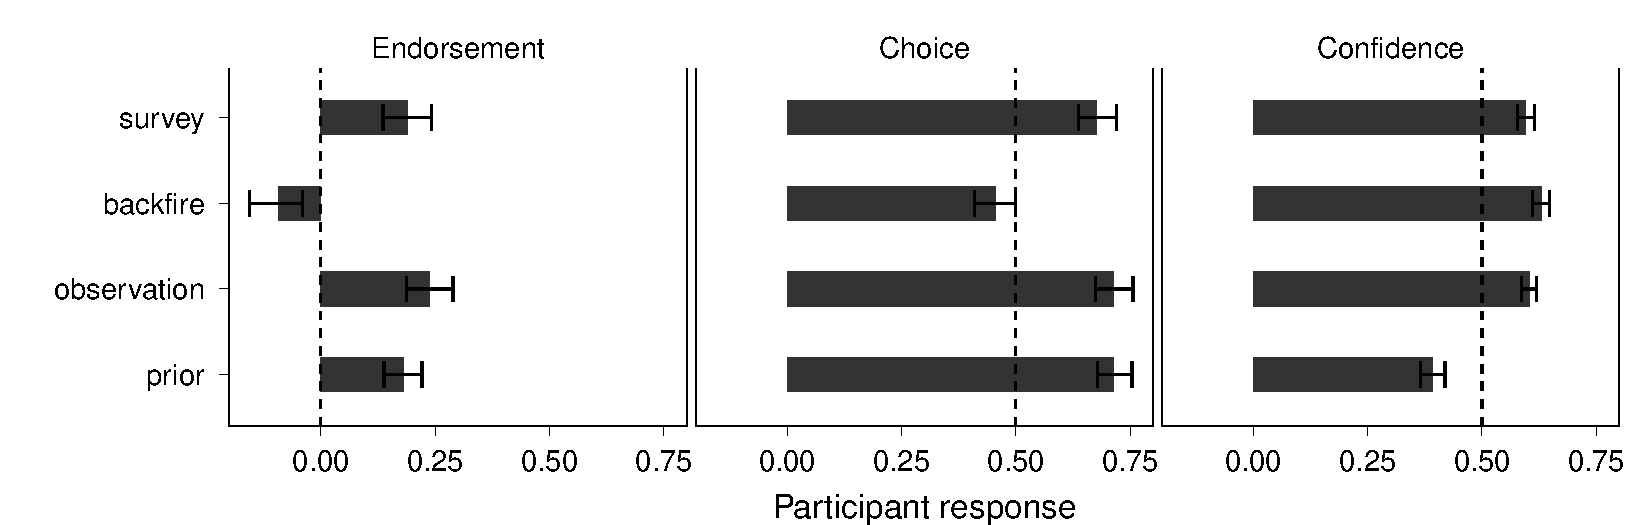
\includegraphics[width=\textwidth]{expt1-3responses}
    \caption{Endorsement scores, forced choice proportions and confidence ratings for each condition in Experiment 1. Dotted lines denote chance levels. Error bars denote bootstrapped 95\% confidence intervals. \mht{need to change condition names}}
  \label{fig:expt1-all}
\end{figure*}



We computed an \emph{endorsement score} by scaling forced-choice responses by their associated confidence level. 
We coded the selection of the more \emph{likely} option (e.g., the student who \emph{always} does turns in his homework on time) as a 1; the other option as -1.
We fit the \emph{endorsement score} data using a generalized mixed-effects model with random by-participant effects of intercept and random by-item effects of intercept and condition\footnote{This was the maximal-model that our data permitted.}. 
As predicted, participants endorsed the likely option \emph{less} in the \emph{Backfiring} condition (M=-0.09; bootstrapped 95\% CI [-0.15, -0.03]) than the in the \emph{Baseline} condition (M=0.18 [0.14,0.22]), $\beta = -0.27; SE = 0.05; t(119) = -5.7; p < 0.001$.
%$\beta = -0.24; SE = 0.03; t(1794) = -8.3; p<0.001$
Participants in the Observation condition (M=0.24 [0.18, 0.29]) and the Instructive condition (M=0.18 [0.13, 0.24]) were not any more likely to endorse the likely option than in the \emph{Baseline} condition ($\beta = 0.06; SE = 0.05; t(119) = 1.25$ and $\beta = 0.006; SE = 0.04; t(119) = 0.15$, respectively). 

%REML criterion at convergence: 2916.7
%
%Scaled residuals: 
%     Min       1Q   Median       3Q      Max 
%-2.81054 -0.56303  0.07179  0.58951  3.12247 
%
%Random effects:
% Groups   Name                 Variance Std.Dev. Corr             
% workerid (Intercept)          0.012651 0.1125                    
%          conditionobservation 0.142176 0.3771   -0.16            
%          conditionbackfire    0.181413 0.4259    0.28  0.61      
%          conditionsurvey      0.113661 0.3371    0.03  0.81  0.64
% item     (Intercept)          0.001253 0.0354                    
% Residual                      0.212359 0.4608                    
%Number of obs: 1920, groups:  workerid, 120; item, 16
%
%Fixed effects:
%                       Estimate Std. Error         df t value       Pr(>|t|)    
%(Intercept)            0.180966   0.025050  77.950000   7.224 0.000000000295 ***
%conditionobservation   0.056732   0.045531 119.020000   1.246          0.215    
%conditionbackfire     -0.273166   0.048983 119.020000  -5.577 0.000000155815 ***
%conditionsurvey        0.006237   0.042856 119.000000   0.146          0.885    
%---
%Signif. codes:  0 ?***? 0.001 ?**? 0.01 ?*? 0.05 ?.? 0.1 ? ? 1
%
%Correlation of Fixed Effects:
%            (Intr) cndtnbs cndtnbc
%cndtnbsrvtn -0.440                
%condtnbckfr -0.271  0.562         
%conditnsrvy -0.405  0.671   0.577 

To better understand the effect, 
we further analyzed the data separately in terms of (1) the proportion of participants who selected the more \emph{likely} option and (2) the confidence ratings.
Critically, participants were significantly \emph{less} likely to choose the likely option in the \emph{Backfiring} condition than at baseline ($\beta = -1.42; SE = 0.15; z=-9.0;$).  % p < .001%
Interestingly, however, participants were \emph{no more} likely to choose the likely option in either the \emph{Observation} or \emph{Instructive} conditions than at baseline (Figure \ref{fig:expt1-all}; middle panel).
% backfiring (M=0.46 [0.41, 0.50]) 
% baseline (M=0.71 [0.67,0.75])
% observation (M=0.71 [0.68, 0.75]) 
% instructive (M=0.68 [0.63,0.71]) conditions than in the Baseline (Figure \ref{fig:expt1-all}; middle panel).
Finally, since participants were not given any helpful information in the \emph{Baseline} condition, we expected the confidence rating data to be lower in this condition than in the three experimental conditions.
In all conditions, this was the case (Figure \ref{fig:expt1-all}; right panel).


%: Prior 0.39 [0.36, 0.42] vs. Observation 0.60 [0.58, 0.62], Ignorant Speaker 0.60 [0.58, 0.61], Backfiring 0.62 [0.61, 0.64] 
Overall, participants in the \emph{Backfiring} condition interpreted utterances as expressing atypical events relative to the other three conditions, replicating \citeA{Kravtchenko2015}.  If an officemate says, ``My student turned in his homework today," then the student must not typically turn in his homework.  However, we also expected participants in the \emph{Observation} and \emph{Instructive} conditions to interpret the target statements as evidence that the relevant behavior \emph{does} typically occur more often than at baseline, which we did not find. 
% Upon reading an observation that a student turned in his homework, for instance, we expected participants to be more likely to believe that the student usually turns in his homework, relative to baseline.  We also expected participants to interpret the statement, ``My student turned in his homework today," as evidence that the student usually turns in his homework when produced in response to a question about whether the student turned in his homework.  Instead, participants in these two conditions did not differ from those in the \emph{Baseline} condition.  
This lack of differences could be due to participants having a strong prior belief that the ``more likely" option given the evidence was also more likely \emph{a priori}: we observed a baseline probability reliably greater than 50\% for 8 out of the 16 items.
Participants also might have interpreted the observation and instructive vignettes as suggestions \emph{from the experimenter} that the habit was unlikely.  Thus, those conditions might have backfired to an extent, as well (e.g., participants might have asked themselves, \emph{why is the experimenter going through all this trouble to tell me that the event occurred?}) \mht{cite ransom et al., experimenter effects in reasoning?}.
We designed the next experiment to get around these issues.

%Two possible explanations for this lack of differences are: 1) prior beliefs could have already been relatively high, making it difficult for linguistic and observational evidence to influence responses, and 2) participants might have needed more than one piece of evidence to make a strong generalization about behavior.

%\red{do we need the median split?  could it be enough to just say, yeah, the observation and ignorant speaker conditions were funky because overall, prior beliefs were pretty high?  and then focus on the most important / interesting topic, which is the backfiring} fact that we observe an effect in the Backfiring condition but not in the other conditions might in fact be expected if the items for which the prior beliefs are the strongest show a relatively small effect of evidence compared to when prior beliefs are the weakest.
%The opposite pattern would be expected for the Backfiring condition, where it is predicted an utterance will backfire the most when the prior beliefs are the strongest (see Figure \ref{fig:schematic-model}) for model predictions).
%To this end, we performed a median split of the items based on their prior endorsement. 
%Figure \ref{fig:expt1-medspilt} shows mean endorsement score in each of the three conditions against the backdrop of the prior endorsement score, when the items are split based on prior endorsement. 
%We see a larger deviation from the prior for the Observation and Ignorant Speaker conditions and a smaller deviation from prior for the Backfiring condition, when the prior is relatively weak. 
%The opposite pattern is observed when prior beliefs are relatively stronger, as predicted by the theory (Figure \ref{fig:schematic-model}). 

%\ndg{think through the best way to analyze / present the relation to prior....}



%    condition      mean  ci_lower  ci_upper
%       (fctr)     (dbl)     (dbl)     (dbl)
%1       prior 0.3923750 0.3643260 0.4193974
%2 observation 0.6030833 0.5833073 0.6184844
%3    backfire 0.6291875 0.6102781 0.6488406
%4      survey 0.5956458 0.5757083 0.6145448



%\begin{figure}
%\centering
   % 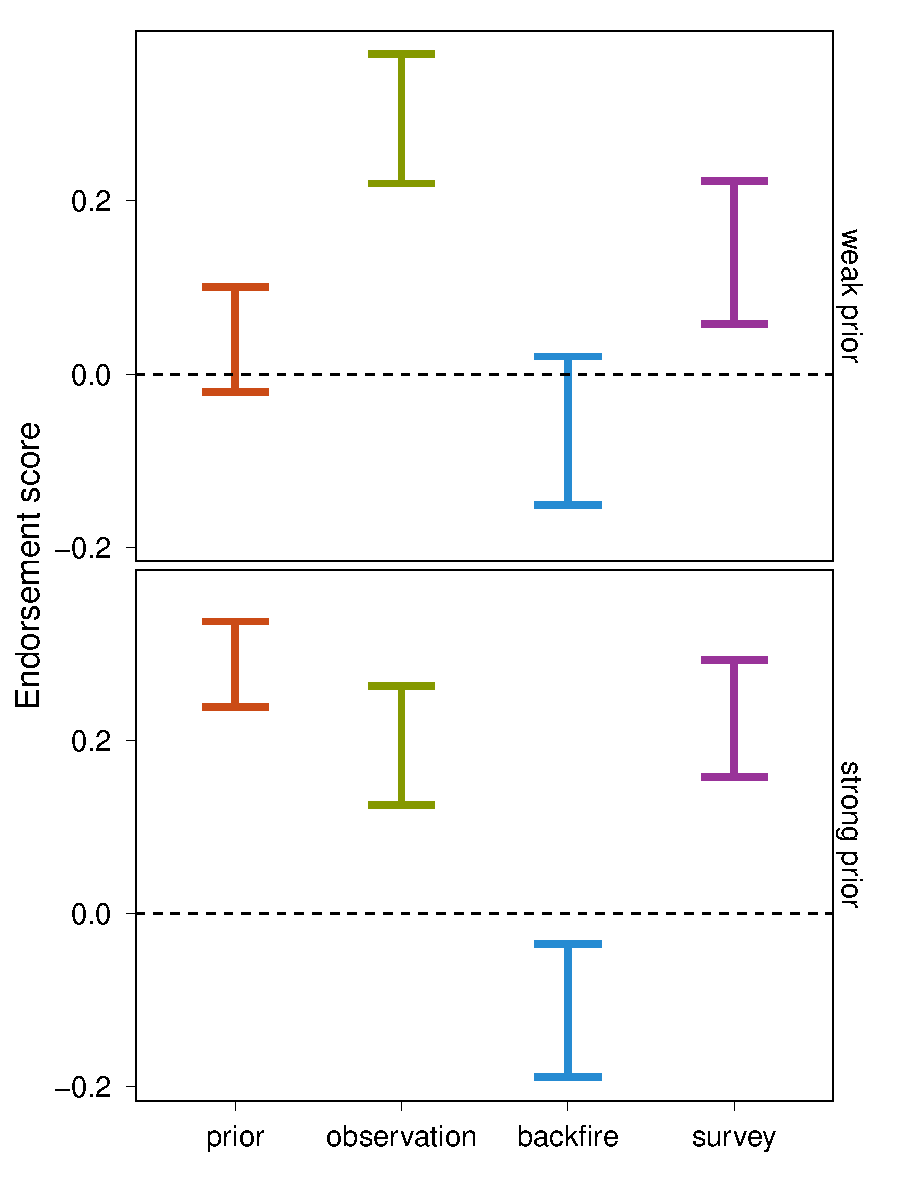
\includegraphics[width=\columnwidth]{fc2-score-medSplit}
    %\caption{Median split of the data based on endorsement score in the Prior condition. 
    %Dotted lines denote mean prior levels with 95\% CIs.}
  %\label{fig:expt1-medspilt}
%\end{figure}







% neither the observational data nor the utterance when common ground is aligned have an effect above and beyond the prior is not surprising \emph{if}  
%
%We were somewhat surprised to \emph{not} find an effect of the observational data or the utterance when common ground is aligned on the endorsement of the more likely response above and beyond the prior endorsement. 
%
%Reading, for example, "My student turned in his homework on time today,"€ in a communicative context caused participants to infer that the student does not typically turn in his homework on time.  
%Adults were also more confident in their choices in the Pragmatic condition (M = .63, SE = XX, n = XX) than in the Baseline condition (M = .39, SE = XX, n = XX).
%
%
%To determine how the Pragmatic, Literal, and Speaker Manipulation conditions compared to the Baseline condition, we fit the data using mixed-effects regression models comparing the responses and confidence ratings of the experimental conditions to those of the Baseline condition.  
%Each model had a fixed effect of condition and random effects of item and participant.  
%To test for the significance of effects, we performed likelihood ratio tests. 
%Chi-squared values, degrees of freedom, and p-values, all from the likelihood ratio test, are reported for each statistical test.
%
%
%The Literal (M = .71, SE = XX, n = XX) and Speaker Manipulation (M = .68,  SE = XX, n = XX) conditions, however, did not differ significantly from the Baseline condition, χ2(1) = 0, p = .98, and χ2(1) = 2.11, p = .15, respectively, even though we expected participants in these conditions to be more likely to choose the "likely"€ option.  One possibility is that for the items in this task, there was not much room for preference for the "likely"€ option to strengthen, given that participants already preferred the "likely"€ option in the Baseline condition at above-chance levels, t(119) = 9.05, p < .001.  Confidence ratings, however, did distinguish among these conditions.  Confidence ratings in both conditions (M = .60, SE = XX, n = XX in the Literal condition; M = .60, SE = XX, n = XX in the Speaker Manipulation condition) were significantly higher than confidence ratings in the Baseline condition,  χ2(1) = 275.41, p <.001, and χ2(1) = 255.68, p < .001, respectively.  Thus, the evidence provided in these two experimental conditions made adults at least more confident in their choices.  
%
%POST-HOC ANALYSES?
%To determine how pre-existing biases might influence participants'€™ responses in each of our conditions, we performed a median split analysis, separating items in the Baseline condition for which participants had weak preferences (M  = XXXX) from those for which participants had strong preferences (M = XXXX).  


%\subsection{Quantitative model evaluation} \red{TAKE OUT?}

%The formal pragmatics model in Eq.~\ref{eq:L1} describes how a listener is likely to interpret an utterance affirming an event, when she believes the speaker to have presupposed some information. 
%Since there is appreciable variability in participants' ratings in the Prior condition, we can use those ratings as $P(h)$ and explore the quantitative predictive power of the model.
%We assume, for simplicity, that the various habits described in the experimental context give rise to their associated behaviors --- $P(b \mid h)$ --- as given in Eq.~\ref{eq:hab}.
%We model the Observation data using Eq.~\ref{eq:bayes}, the Misaligned CG data using Eq.~\ref{eq:L1} and the Aligned CG data using Eq.~\ref{eq:L1mod}.

%The model has one remaining parameter: the speaker optimality parameter in Eqs.~\ref{eq:S1} and \ref{eq:S1mod}. 
%We assume these two parameters are the same in this analysis, and infer its credible value using Bayesian data analytic techniques \cite{LW2014}. 
%The posterior predictive distribution marginalizes over the likely parameter values to produce predictions about what the data should look like given the pragmatics model and the observed data. 
%This is akin to fitting the parameters and is an important step in model validation as it shows what data is actually predicted by the model.
%We compare the posterior predictive distribution over the probabilities of producing the \emph{likely} response to the empirical means for each item and condition (Figure \ref{fig:scatter}). 
%The model provides a reasonable quantitative fit to the empirical data ($r(48) = 0.82$), though the fit is far from perfect.

%One issue is that there is not an a lot of reliable variability in the human judgments within the different conditions, most notably in the Misaligned CG condition. 
%We also seem to be doing the worst job capturing the data from the Observation condition using Eq.~\ref{eq:bayes}. 
%This may be an artifact of the task: In order to present observational data to the participant, we used extended vignettes to explain how the protagonist was able to notice the event occur. 
%Such an elaborate cover story may have raised the question to the participants of why the experimenter to choosing to supply this information. 
%This may inadvertently have led to a \emph{backfiring} effect for some of the items.

%\ndg{is it possible to get a wider range of predicted values from the (unaligned) model? if so, it would be worth running the corresponding experiment....}

%\begin{figure}
   % 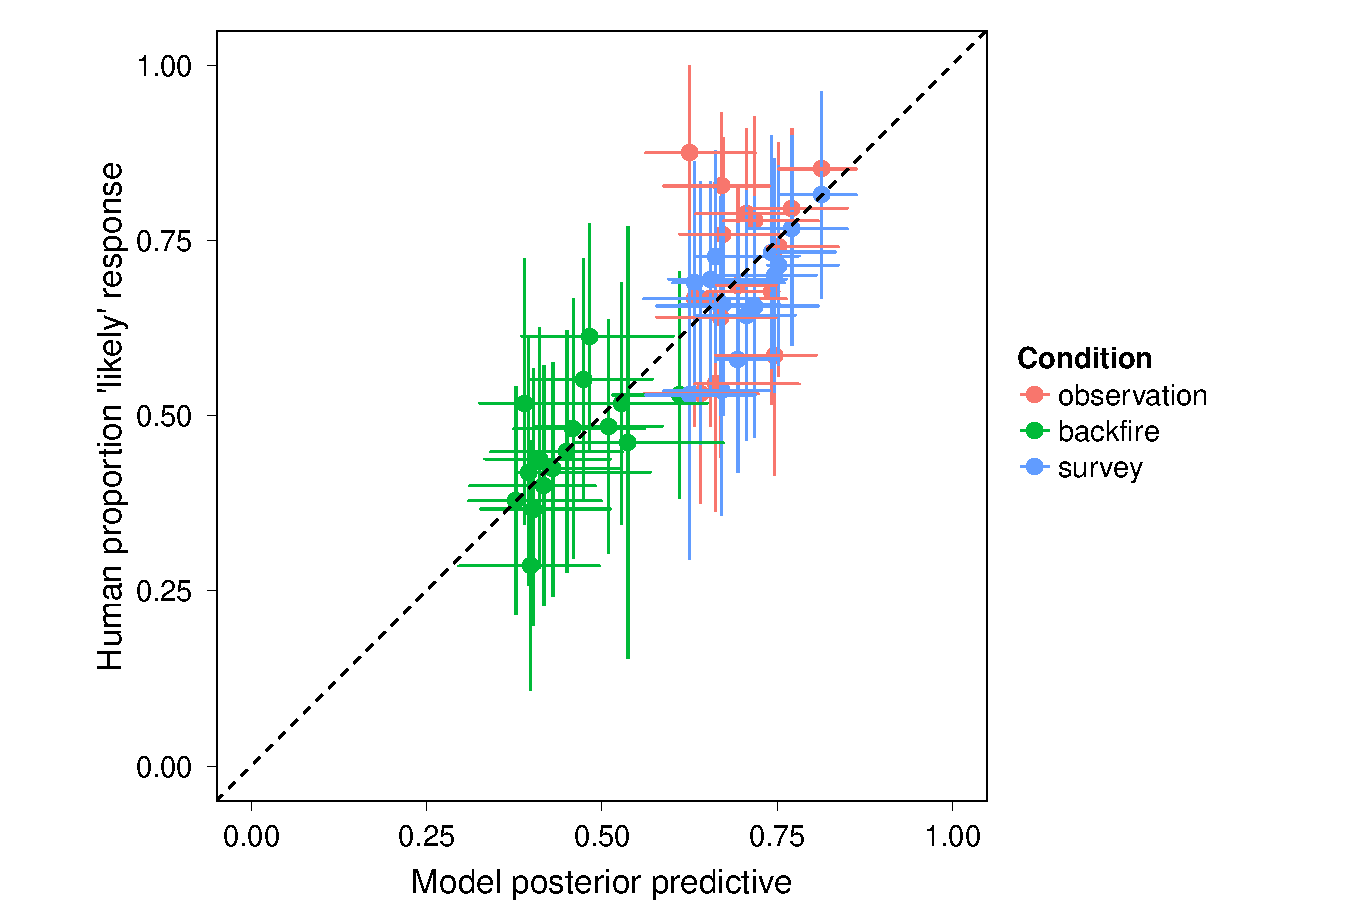
\includegraphics[width=\columnwidth]{scatter}
    %\caption{Model predictions and the associated human endorsements.}
  %\label{fig:scatter}
%\end{figure}


%\section{Experiment 2} 
%Experiment 1 demonstrated the existence of a backfiring effect as a speech-act of what would usually be construed of as positive evidence: the observation of an event. 
%In Experiment 2, we explore downstream consequences of this inference. 
%If intuitive, structured theories of world are what guide inference, then we would expect to observe the effects of backfiring in different components of that structured konwledge.
%For example, If habits have a causal dependence on some more abstract trait, then having one's belief shaken in a person's habit can have belief shaken in the upstream trait. 
%For instance, upon hearing one's friend say \emph{My roommate did her dishes today.}, a hearer could plausibly infer both this an irregular event and that the roommate is the kind of person who wouldn't normally do her dishes. 
%That is, the roommate's room might also be a mess, she might be an inconsiderate person, or maybe more likely than not to fall delinquent on her rent checks.

%This opens the door for manifestly different types of conceptual learning from language. \red{This is a good point, but I feel like we'll end up focusing *not* on language (and instead on the relation between irregular events and traits)... which maybe is ok, I don't know.}


%
\section{Experiment 2: Degrees of backfiring}

\begin{figure*}
%\centering
    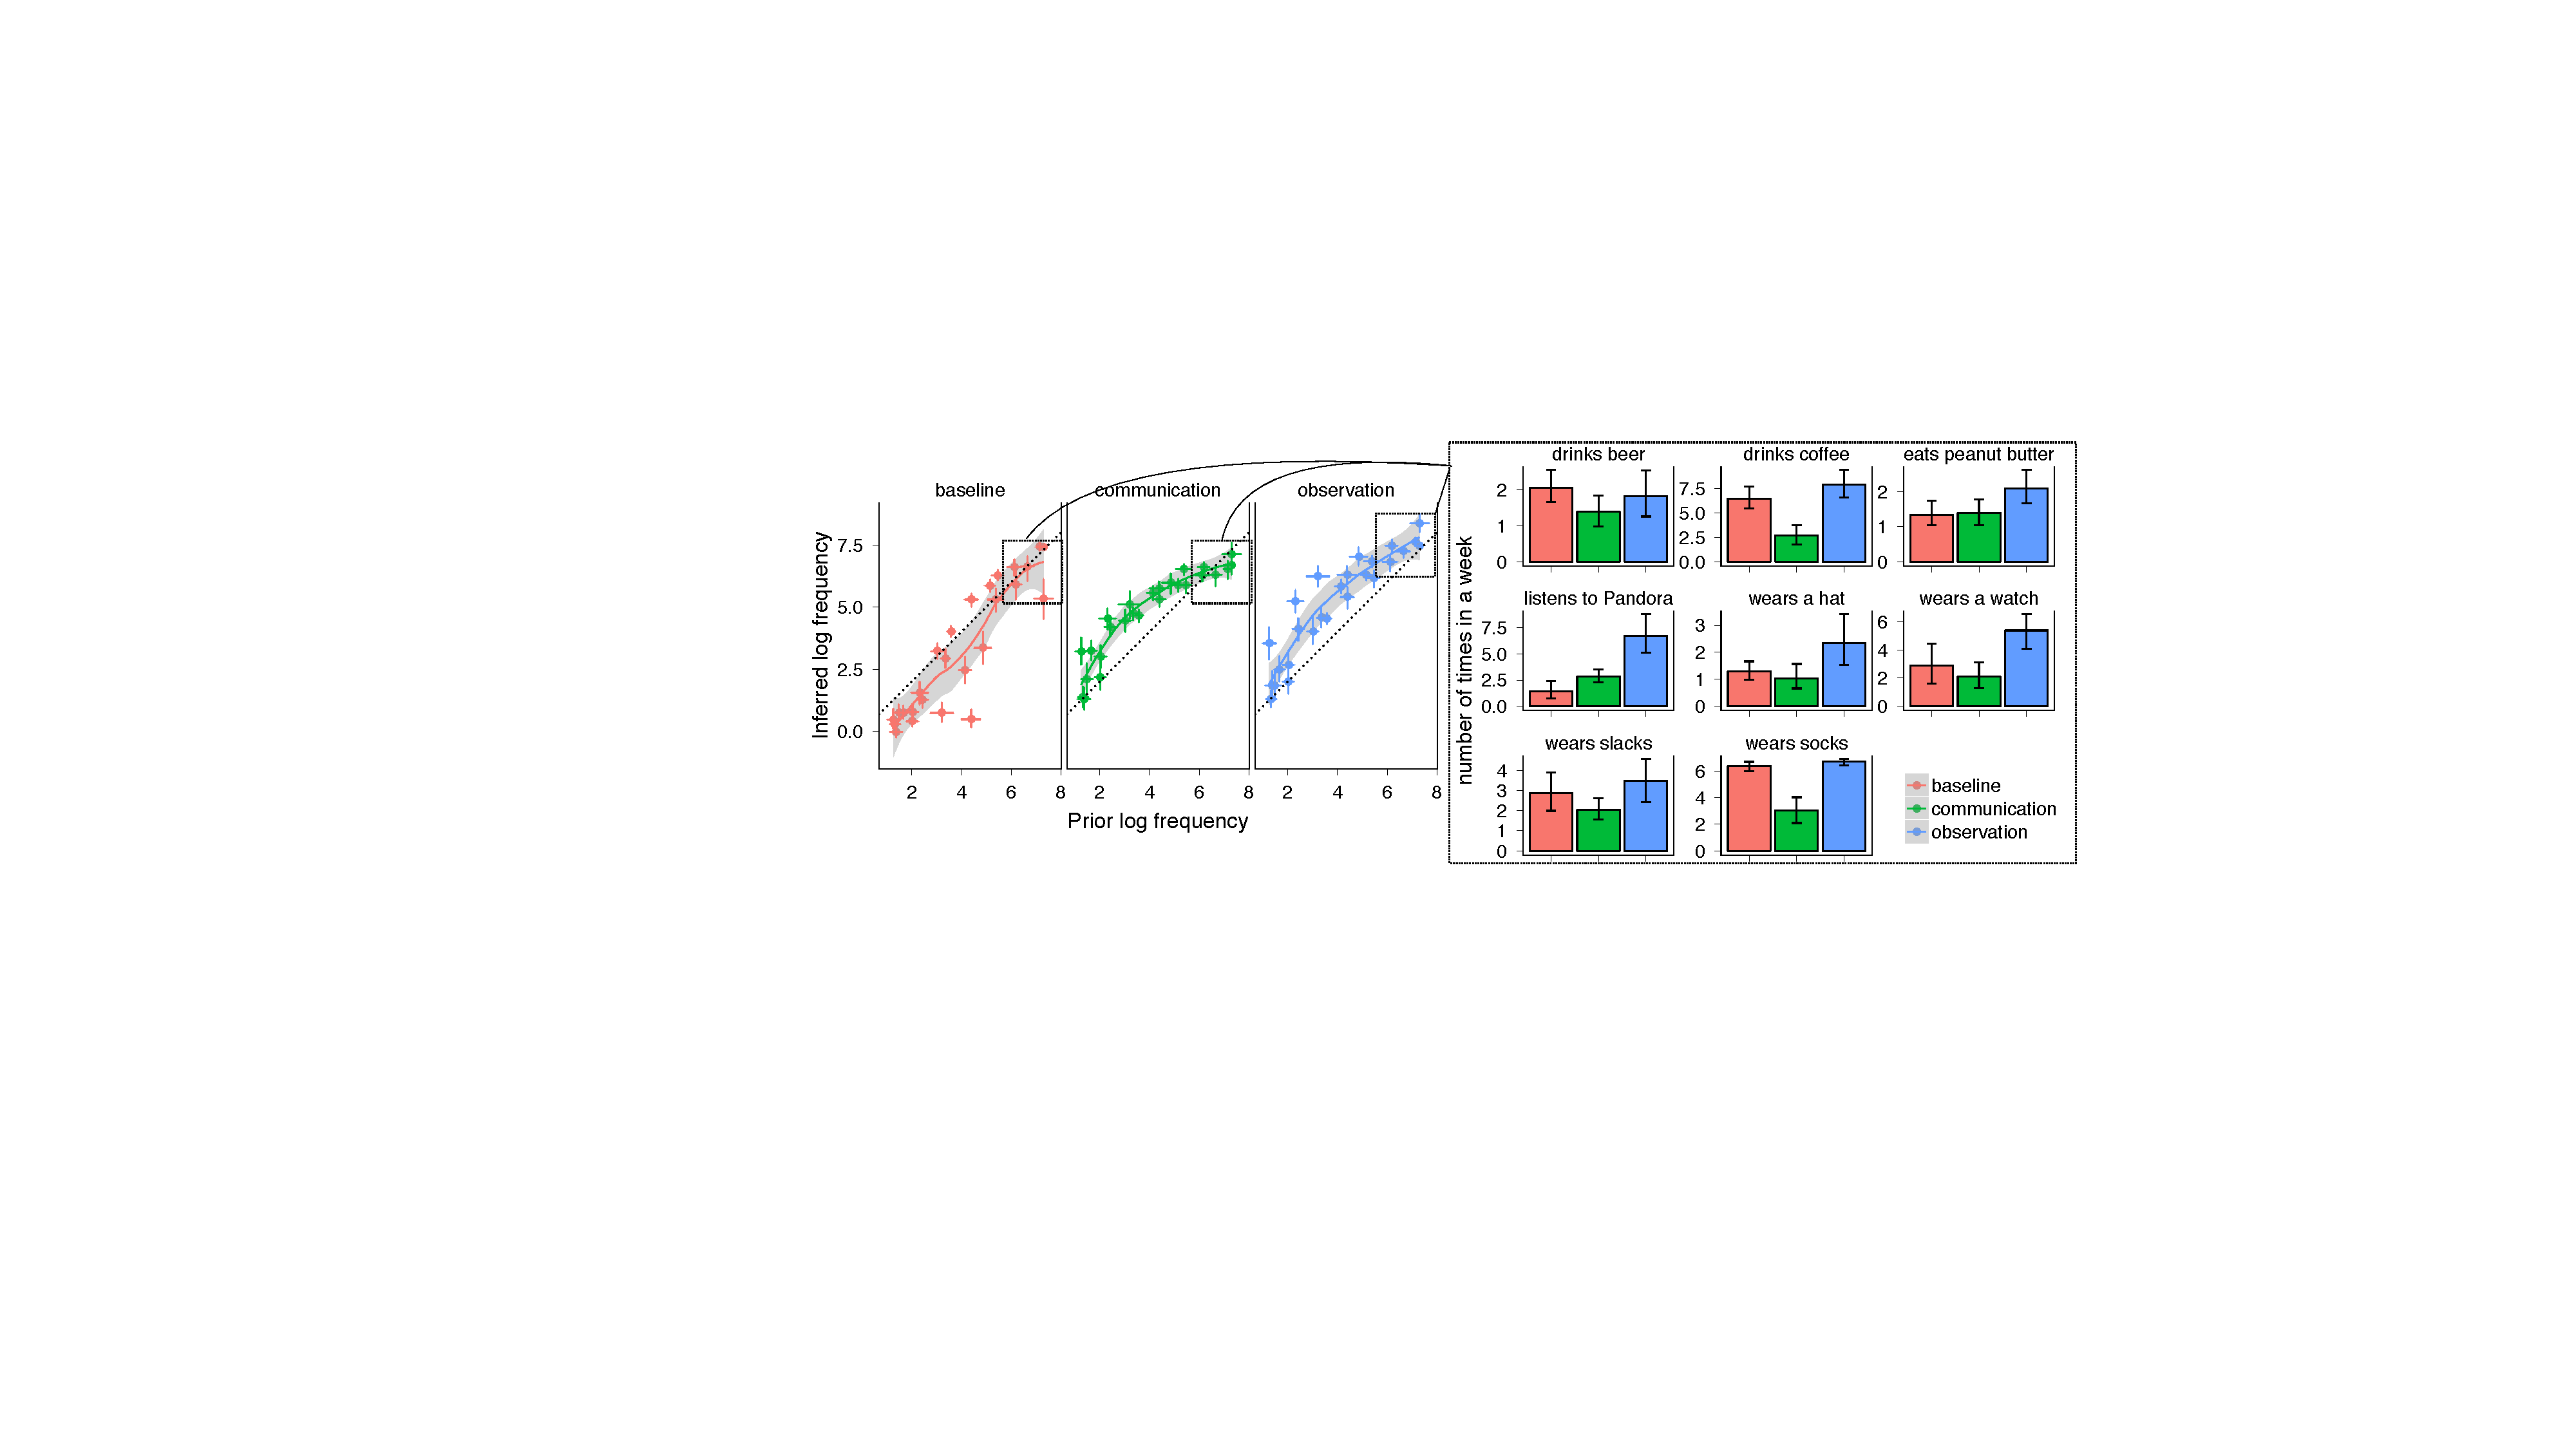
\includegraphics[width=\textwidth]{expt2-scatter-witems}
    \caption{
    Left: Inferred frequency as a function of \emph{a priori} frequency (see text) for the three experimental conditions. In only the communicative condition, does the inferred rate dip below the prior rate. Both axes are on the log scale.
    Right: Item plots in the region of interest. When the \emph{a priori} frequency is high, backfiring effects are the largest. 
    }
  \label{fig:expt2}
\end{figure*}


The model of backfiring language (Eq. \ref{eq:L1}) predicts that the extent to which backfiring should occur depends upon the \emph{a priori} likelihood of the action occurring. 
In our second experiment, we aimed to elicit reactions to utterances about human behaviors that vary widely in terms of this likelihood.

%human behaviors covering a wide range of likely frequencies of action, as well as to simplify and generalize the experimental paradigm. 
%modified the stimuli used in Experiment 1 to include actions associated with a wider range of prior beliefs so that we could test the quantitative predictions of our models. 
%Specifically, we ask whether the strength and presence of backfiring varies systematically according to the strength of prior beliefs. 
Specifically, our model predicts that the degree of backfiring should vary \emph{continuously} according to the \emph{a priori} likelihood of the event, with strong backfiring for utterances about events that are \emph{a priori} very likely (e.g., ``John wore socks today") and either weaker or no backfiring for events that are very \emph{un}likely (e.g., ``John climbed a mountain today"). 

%\red{OR:} In our second experiment, we modified the stimuli used in Experiment 1 to include actions associated with a wider range of prior beliefs so that we could test the quantitative predictions of our models.  Specifically, we asked whether the strength and presence of backfiring varies systematically according to the strength of prior beliefs.  Our models predict that utterances that are strongly redundant with prior beliefs (e.g., ``John wore shoes today") should backfire more than utterances that are less redundant (e.g., ``John went for a hike today"), by virtue of being less semantically informative.

\subsection{Method}

\subsubsection{Participants}
Participants were 150 workers from Amazon's Mechanical Turk platform. 
All had at least a 95\% work approval rating.
The task took about 7 minutes and participants were compensated \$0.80.

\subsubsection{Materials and procedure}
Participants were randomly assigned to one of three conditions: the \emph{Backfiring} condition, the \emph{Observation} condition, or the \emph{Baseline} condition.

In the \emph{Observation} condition, participants were told that on each trial they would be given a random fact about a person, and then be asked to judge how often that person performs the action.  Each trial had the same format: ``\textsc{person} did X today'', where X was an action (e.g., ``Stephen went for a run today.'').  Participants were then asked, ``How often does \textsc{person} do X?''  (e.g., ``How often does Stephen go for runs?'').  Participants responded ``M times per K,'' by entering a number for M and choosing K from a drop-down menu with options for \emph{week}, \emph{month}, \emph{year}, and \emph{5 years}. 

In the \emph{Backfiring} condition, participants were instead told that they would read excerpts from conversations between friends.  
On each trial, participants read, ``You overhear two friends talking. One of them says to the other, `\textsc{person} did X today'.''

In the \emph{Baseline} condition, participants were asked to rate how often a typical person performs the action, without having read any other information.

Before the task and after reading the instructions, participants were asked what they would do in the task, and were given a drop-down menu with 4 options, 3 of which summarized the instructions above and one of which was a distractor. 

%were asked to select from a
%  We asked participants to assume that the typical person had performed the action at least once, so that the priors / to avoid the possibility that... \red{we should justify why we used the exact baseline we did}
%
%consisted of a single utterance: one person describing an event to a friend (e.g., ``Kelly wore socks today").  After reading each utterance, participants indicated how frequently they believed the agent in the utterance engages in the activity (e.g.,``How often does Kelly wear socks?").  Participants responded by stating \emph{X} times per week, month, year, or five years, where \emph{X} could be any number.

\subsection{Prior data}

As a basis of comparison and for estimation of the prior distribution for the quantitative model fit, we use previously collected data from an unrelated experiment as a measure of the prior. 
In this prior elicitation task (reported in full in Tessler \& Goodman (\emph{CogSci 2016}, submitted)), 40 MTurkers rated how often a person who has done the action (e.g. \emph{smoked cigarettes}) at least once, does the action. 
The response format was the same as in Expt.~2. 

%We then modeled the data from each of the \emph{Backfiring} (Eq.~\ref{eq:L1}), \emph{Observation} (Eq~\ref{eq:bayes}), and \emph{Baseline} conditions (Eq.~\ref{eq:bayes} neglecting the evidence) of Expt.~2.
%\subsubsection{Prior data}
%rated how often a person who has done the action (e.g. ``smoked cigarettes'') at least once, does the action. 
%Participants answered this question for both men and women independently. 
%From this data, we can estimate the likely rates that gave rise to the count data measured using Bayesian data analytic techniques. 
%Because the participant was only told that the target person had done the action \emph{once}, we assumed that each item had two components corresponding to individuals who do the action \emph{relatively frequently} (with rate $\lambda_h$) and those who do the action \emph{relatively infrequently} (rate $\lambda_{\neg h}$).
%These two components came together with mixture parameter $\theta$ inferred from teh data.
%The data is thus distributed as: $d_{prior} \sim \theta \cdot \text{Poisson}(\lambda_{h}) + (1 - \theta) \cdot \text{Poisson}(\lambda_{\neg h})$.
%



\subsection{Behavioral results}

Twenty-two participants were excluded from the analyses for failing the instructions comprehension trial.\footnote{
15 of the 22 excluded participants were from the Observation condition, and 14 out of those 15 selected the instruction summary from one of the other conditions (i.e., only 1 selected the distractor). This may be a result of the instructions in the Observation condition being relatively generic.
}

We analyzed the data by normalizing the elicited rates to the scale of numbers of times in a 5 year period (the maximum time window). We then log-transformed the rates. 
Figure \ref{fig:expt2} (left) shows the inferred rates on a log scale compared to the prior elicitation data (also on log scale) described above.
Only in the \emph{Backfiring} condition do the inferred rates drop below the prior. 
Figure \ref{fig:expt2} (right) shows item-specific plots on a normal rate scale  from the high-prior region of interest. 
In some cases (e.g. \emph{wears socks}), the inferred rate is less than 50\% of the \emph{baseline} rate.

To get a better idea for the reliability of this effect with our items, we compared the rate implied by the utterance in the \emph{Backfiring} condition to the rate implied in the \emph{Observation} condition, as a function of the baseline rate.
%
% number of times in a day. For example, if a participant rated that a target person goes on a hike once a month, that was normalized to the daily rate of 0.03.  
We first computed the mean rate from the \emph{Baseline} condition and used that as a predictor (after centering) crossed with condition (Backfire vs. Observational) in a mixed-effects linear regression, with random by-participant effects of intercept and base rate and by-item effects of intercept and condition\footnote{This is the maximal mixed-effects structure.}. 
The frequencies implied in the \emph{Observation} condition were significantly larger than those implied in the \emph{Backfiring} condition ($\beta = 0.35, SE = 0.13, t(67.6) = 2.56, p = 0.01$), and there was a trend for that difference to increase as the base rate increased ($\beta = 0.09, SE = 0.05, t(60.4) = 1.92, p = 0.059$). There was also a significant main effect of base rate on the implied rate ($\beta = 0.57, SE = 0.09, t(27.1) = 6.6; p<0.01$). \red{what does this mean?}
The fact that the effect in our data is small is likely driven by the fact that we have few items in the critical region where we would expect backfiring to occur. 

%We observe a main effect of base rate on the implied rate 
%Because the elicited frequencies cover a wide range 
%After centering the predictors, we observe a main effect of baseline rate ($\beta = 1.32; SE = 0.18; t(25) = 7.1; p <0.001$), meaning that as the baseline rate increases so too do the rates in the observation and backfiring conditions. We also observe a main effect of condition ($\beta = -0.24; SE = 0.05; t(75) = -4.3; p <0.001$), with the backfiring condition in general implying a lower rate than the observation condition. Crucially, we observe an interaction between baseline rate and condition ($\beta = -0.85; SE = 0.12; t(1975) = -7.08; p <0.001$), with the backfiring condition having a lower implied rate than the observation condition, with the difference growing \emph{as the baseline rate increases}. 

%Linear mixed model fit by REML t-tests use Satterthwaite approximations to degrees of freedom [
%lmerMod]
%Formula: daily_prob ~ cbase_rate * ccondition + (1 | workerid) + (1 |      item)
%   Data: cent
%
%REML criterion at convergence: 5873.2
%
%Scaled residuals: 
%    Min      1Q  Median      3Q     Max 
%-3.3280 -0.1836 -0.0161  0.0742 17.7636 
%
%Random effects:
% Groups   Name        Variance Std.Dev.
% workerid (Intercept) 0.02179  0.1476  
% item     (Intercept) 0.10979  0.3313  
% Residual             0.93782  0.9684  
%Number of obs: 2079, groups:  workerid, 77; item, 27
%
%Fixed effects:
%                        Estimate Std. Error         df t value         Pr(>|t|)    
%(Intercept)              0.39900    0.06928   28.00000   5.759 0.00000351692557 ***
%cbase_rate               1.32026    0.18600   25.00000   7.098 0.00000019343954 ***
%ccondition               0.23706    0.05525   75.00000   4.291 0.00005244157717 ***
%cbase_rate:ccondition    0.84899    0.11985 1975.00000   7.084 0.00000000000194 ***
%---
%Signif. codes:  0 ?***? 0.001 ?**? 0.01 ?*? 0.05 ?.? 0.1 ? ? 1
%
%Correlation of Fixed Effects:
%            (Intr) cbs_rt ccndtn
%cbase_rate  0.000               
%ccondition  0.000  0.000        
%cbs_rt:ccnd 0.000  0.000  0.000 

%The backfiring effect can be observed in a number of ways.
%We would have evidence for backfiring if the rate implied by the utterance in a communicative context is:
%\begin{enumerate}
%\item Less frequent than not knowing anything about the person (Backfire vs. Baseline)
%\item Less frequent than you would think had you \emph{observed} the event (Backfire vs. Observation)
%\item Less frequent than not knowing anything about the person except that they have done it at least once in the past.\footnote{The distinction from (1) is potentially important for items such as ``smokes cigarettes'', wherein the typical person (Baseline) may not smoke at all. 
%This may be only subtly different from (2).
%}
%\end{enumerate}
%
%To test 

%\item Less frequent that someone who ``Does X'' (habitually; e.g. ``John smokes'' vs. ``John smoked a cigarette today.'', not measured)


\begin{figure*}
%\centering
    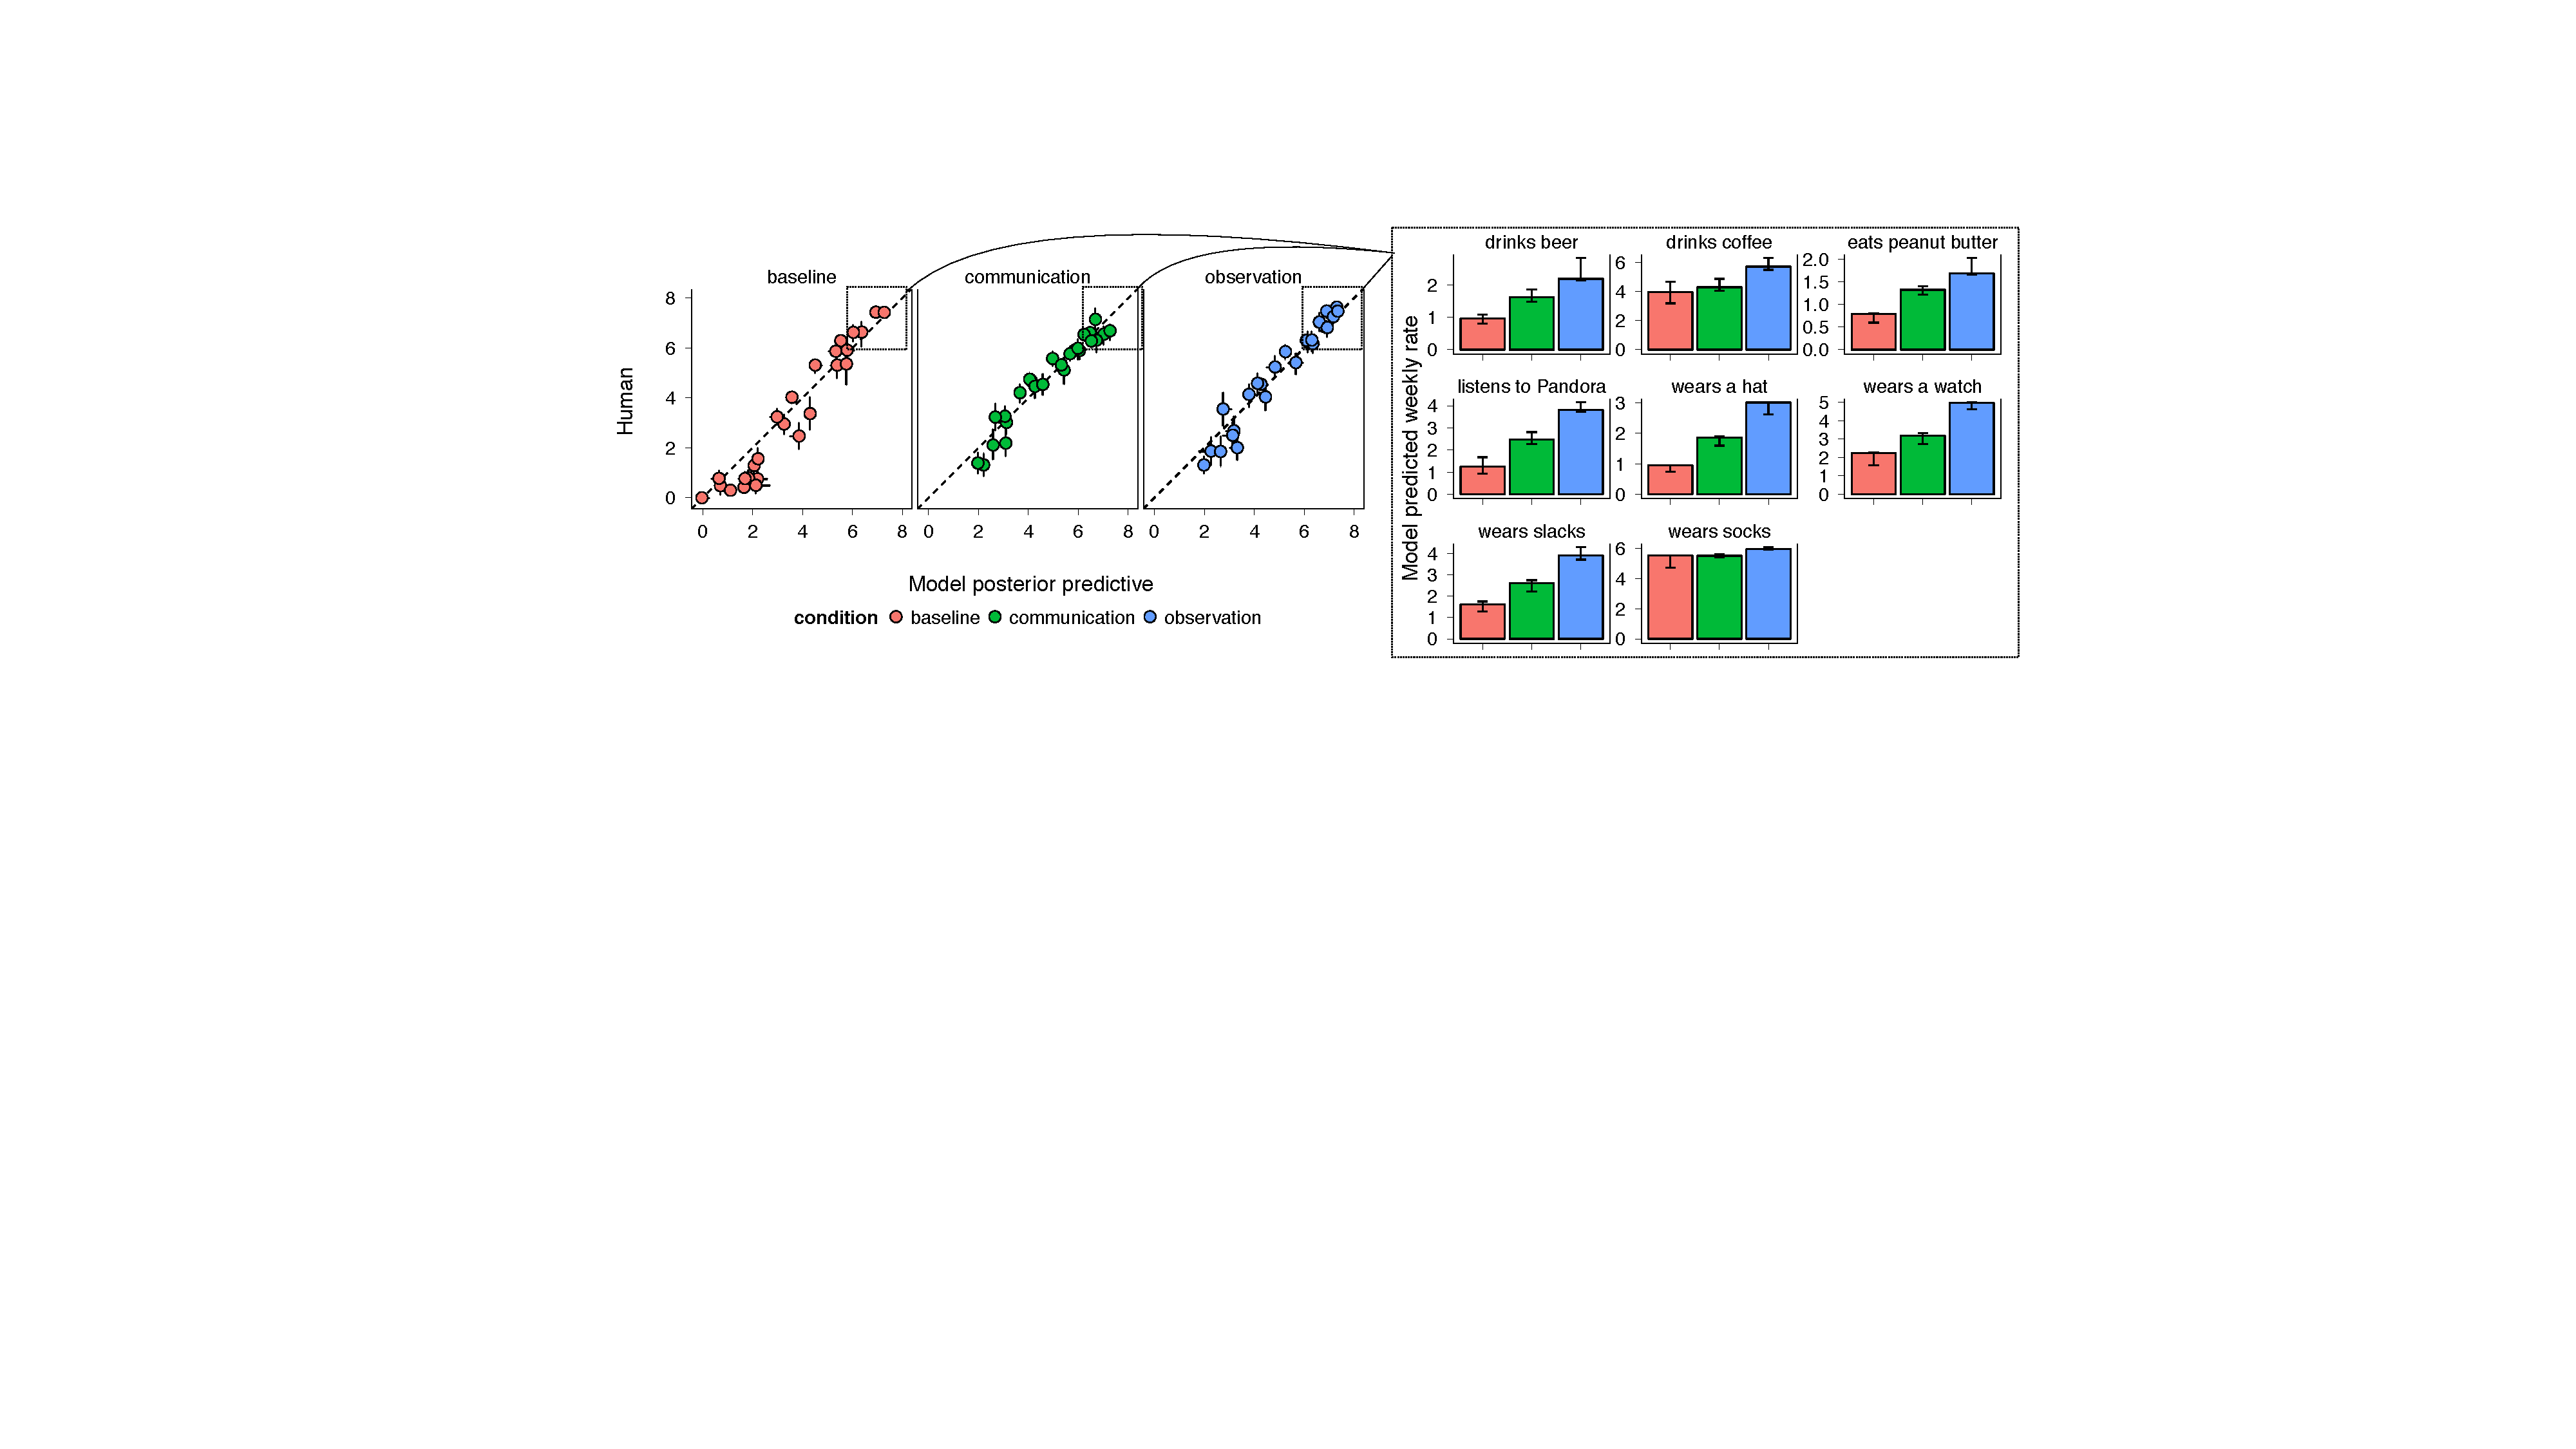
\includegraphics[width=\textwidth]{expt2-scatter-model-witems}
    \caption{
    Left: Model predictions as compared against the human elicited frequencies. Right: Predictions for items in the region of interest.
    }
  \label{fig:expt2model}
\end{figure*}


\subsection{Quantitative model analysis}

In order to quantitatively compare the models to the empirical data, we needed to measure the prior distribution over habits $P(h)$ and the habit strength $P(h \mid b)$. 
We use previously collected data from an unrelated experiment (decscribed above). We then modeled the data from each of the \emph{Backfiring} (Eq.~\ref{eq:L1}), \emph{Observation} (Eq~\ref{eq:bayes}), and \emph{Baseline} conditions (Eq.~\ref{eq:bayes} neglecting the evidence) of Expt.~2.

\subsection{Prior data}
In the prior elicitation task (reported in full in Tessler \& Goodman (\emph{CogSci 2016}, submitted)), 40 MTurkers rated how often a person who has done the action (e.g. ``smoked cigarettes'') at least once, does the action. 
As well, they rated the frequencies of people who had done the action (e.g. ``smoked cigarettes'') before. This procedure is thought to get at two major components in the prior distribution over frequency of action. 
We model the first question as a log normal distribution ($\ln d_{Q1} \sim \text{Normal}(\mu, \sigma) $), and the second as a Beta ($ d_{Q2} \sim \text{Beta}(\gamma, \delta)$).
\mht{If the rest is kosher, I'll explain in better detail. I did the exact same thing with the prior that I did for habituals.}

\subsubsection{Model details}
\mht{This is a sketch. If it is all kosher, I'll write it up in more detail.}

The listener in the RSA model has uncertainty about the actor's propensity to take part in an event (i.e., the strength of his habit). We connect this latent, real-valued habit (which is on the log 5-year frequency scale) to the probability of the event occurring in a day using a logistic function with parameters $k$ (scale) and $m$ (offset). 
$$
f(x) = \frac{1}{1 + e^{(-k*(x-m))}}
$$
We put priors on these parameters $k \sim \text{Uniform}(0, 10)$ and $m \sim \text{Uniform}(-20, 20)$ and infer their credible values with Bayesian data analysis. 
The RSA model has 1 other parameter: the speaker optimality parameter $\alpha$ in Eq.~\ref{eq:S1}, and the Bayesian observation model has 0 more parameters. 

\subsubsection{Model comparison}

%1    logistic_offset    NA 10.5545683 10.6844495  9.7925498
%2     logistic_scale    NA  0.8567678  0.8630608  0.8471872
%3 speaker_optimality    NA 19.3929040 19.9663293 11.8387894

I ran 2 MCMC chains with 100,000 iterations discarding the first 50,000 for burnin. 
The MAP estimate and 95\% HDI for $\alpha$ is 19.3 [11.8, 19.9].
The logistic scale parameter $k$ 0.86 [ 0.85, 0.86] and offset parameter $m$ 10.5 [9.8, 10.7].

The posterior predictive distribution predicts the data well: $r^2(81) = 0.95$.
As well, for items in the region of interest (Figure \ref{fig:expt2model} right), the model predicts backfiring in the communicative but not in the observational context. 
%We include in our data analysis model an alternative model of the data generating process: random behavior. This sub-model explains data points that deviate largely from our models and is important to include to get reliable es

%
%\begin{minipage}{0.5 \textwidth} \small
%	\begin{align*}
%		d_{prior} \sim \begin{cases}
%\text{Poisson}(\lambda_{h})  & \text{if } h\\
%\text{Poisson}(\lambda_{\neg h})  & \text{if not } h
%\end{cases} \label{eq:hab}
%%		
%%		&\sim \text{Poisson}(\lambda_{h}) \\
%%		\         &\sim \text{Poisson}(\lambda{\neg h}) \\
%	\end{align*}
%\end{minipage}



\section{General Discussion}

We have presented a formal model for how an utterance can \emph{backfire}, or imply that its stated content is typically not true.
%a phenomenon wherein the explicit meaning of a sentence is accompanied by an implication that the sentence is typically not true.
The model is based on the notions that 1) utterances are intended to be informative, and 2) a speaker will assume a body of shared knowledge, or common ground, with a listener.  When a listener hears a speaker say something that seems, on the surface, uninformative, she will adjust her understanding of what must have been presumed to be in common ground to \emph{make} the speaker's utterance informative.  Thus, after hearing, ``My roommate washed her dishes today," a listener who does not know the roommate should infer that the roommate does \emph{not} typically wash her dishes.

%We present a formal model for understanding of \emph{backfiring}, a phenomenon wherein the explicit meaning of a sentence is accompanied by an implication that the sentence is typically not true.
%The model derives predictions by revising common ground between interlocutors so that a speaker's utterance is always informative.  After hearing, ``My student turned in her homework," for example, the model predicts that a person who does not know the student should infer that the student does \emph{not} typically wash her dishes.

%In Expt.~1, we validate that this prediction depends on the information being communicated \red{not sure what this means} as well as a misalignment of common ground between speaker and listener in conversation. This experiment also serves as a conceptual replication of \citeA{Kravtchenko2015} and adds to the body of literature demonstrating that adults try to avoid redundancy in conversation (CITE).
%Ultimately, this can result in an utterance ``backfiring",.  If a person notes, ``My roommate washed her dishes today," for example, then a listener who does not know the roommate will likely infer that the roommate does \emph{not} typically was her dishes; otherwise, the utterance would not be informative (CITE).



Our model also makes several novel predictions about backfiring, which we tested in Experiments 1 and 2.  In Experiment 1, after replicating the basic backfiring effect found by \citeA{Kravtchenko2015}, we showed that this effect disappears when an interlocutor elicits the target utterance by genuinely expressing uncertainty.  If a person taking a survey asks their friend, ``Did your roommate wash her dishes today?" because she needs to answer a survey and the friend responds, ``Yes, my roommate washed her dishes today," then the utterance no longer presupposes any shared knowledge about the roommate; instead, the utterance is clearly established as semantically informative for the listener.  The effect also disappears when the proposition is framed as an observation rather than a communicative utterance (e.g., ``She saw that the roommate washed her dishes today").  In these contexts, there is no longer any pressure for statements to be maximally informative.  As a result, even if the statement is redundant with adults' prior expectations, adults will accept the statement as evidence that the behavior usually occurs.  In Experiment 2, we demonstrated that the existence and strength of backfiring depends on the strength of prior beliefs.  For example, for a person who does not know Jane, the utterance, ``Jane wore shoes today," will result in stronger backfiring than, ``Jane wore sandals today," because wearing shoes more strongly \emph{goes without saying}.

Ultimately, our experiments contribute to the growing body of work on presupposition \red{(CITE)}.  
Traditionally, it has been assumed that information can be presupposed only if it is already part of the common ground between speaker and listener \red{(CITE)}.  Several researchers have argued, however, that an utterance can be perfectly felicitous even if it presupposes information that the listener does not already know \red{(CITE)}.  For example, for a speaker to assert \emph{It was Percival who piqued the professor}, the speaker must believe that the listener already knows that \emph{somebody} had piqued the professor \cite{Clark1977}.  But if the listener actually lacks this knowledge, the exchange does not fall apart; instead, the listener easily and rapidly \emph{accommodates} the utterance by adjusting the common ground between herself and the speaker, inferring that it must be commonly known that someone had piqued the professor.  Here, we argue that listeners engage in a similar process when an utterance seems to be uninformative (e.g., ``John wore shoes today").  In this case, the listener accommodates the speaker by accepting as true a world in which John does not typically wear shoes.  Presupposition is thus a powerful way of communicating information.  %When a speaker presupposes information, given that the speaker is trustworthy, the speaker requires the listener to accept that information as true; otherwise, the speaker's utterance would be uncooperative \cite{Grice1975}.


%\red{points:}

%\red{ - conversation is fraught with misunderstandings - how do we navigate them?}

%\red{ - misunderstandings don't have to result in conversation breaking down - instead, adults readily accommodate each other, or infer the information that should be in common ground for the utterance to make sense.  so, basically, adults are prepared to rapidly convert misunderstandings into understandings.}

%\red{- this process ultimately makes presupposition accommodation extremely powerful - the information is implicitly communicated, and, given that the speaker is trustworthy, the listener is basically forced to accept a world in which the utterance is cooperative.  several studies - loftus and palmer, etc. - have demonstrated the remarkable power of presupposition.  THUS, this work has plenty of practical relevance, and should be considered by people trying to convince society to change its mind about something...}




%\mht{I think we should scrap this paragraph, which is a restatement of things we've said earlier, in lieu of a deeper discussion about accommodation and presupposition}
%\red{ekc: ok, well some of that could be things that we removed from the introduction.  we originally had good examples in there of presupposition and accommodation, including the percival example, and could put that here instead.  but i think we do need at least a short summary of our novel findings - not just the model.}

%\red{cut from intro: Although interlocutors often directly manage information that is in common ground by expressing lack of understanding, they can also use the conversational principle that utterances should be both relevant and informative \cite{Grice1975} to infer the knowledge that a speaker is presupposing in a given utterance.
%For example, for a speaker to assert \emph{It was Percival who piqued the professor}, the speaker must believe that the listener already knows that \emph{somebody} had piqued the professor \cite{Clark1977}.  But if the listener actually lacks this knowledge, the exchange does not fall apart; instead, the listener can accommodate the utterance by adjusting the common ground between herself and the speaker, inferring that it must be commonly known that someone had piqued the professor (von Fintel?).}
%Our experiment serves as a conceptual replication of \citeA{Kravtchenko2015}.
%Our work expands upon theirs in the following ways: 
%(1) We include control conditions that show how the information is interpreted when it is an observation as well as when it is an utterance when common ground is aligned between speaker and listener; 
%(2) We show how the strength of the inference depends systematically on the strength of the prior;
%(3) We include a formal pragmatics model that predicts all of the above.

%presented a formal model for Common Ground inference that uses communicative principles (\emph{be truthful}, \emph{be informative}) to infer what presuppositions the speaker must have brought to conversation. 
%The model predicts that an utterance that should ``go without saying'' given one Common Ground will lead a listener to infer a different Common Ground, and result in a backfiring effect decreasing the listener's belief in the proposition being affirmed.
%The quantitative model predicts that this effect should be strongest when the \emph{a priori} beliefs in the common ground that would make the utterance uninformative are the strongest.
%This is in contrast to typical Bayesian updating, where the most information is gained when \emph{a priori} beliefs are most uncertain. 
%We validate all of these predictions in our experiment.

%We replicate previous findings that adults revise their beliefs about information that is in common ground between interlocutors so that utterances are not redundant with the preexisting beliefs of the listener (CITE).  This revision of beliefs ultimately undermines the literal content of the utterance.  Upon hearing, "My student turned in his homework on time today," for instance, adults will learn that the student turned in his homework on time, but they will also infer that the student must not \emph{typically} turn in his homework on time.



%we developed a computational model that predicts this behavior; 2) we demonstrated that adults do \emph{not} make this inference when the listener's uncertainty about the event is in common ground with the speaker, or when the utterance is removed from a conversational context (i.e., when it is framed as an observation); and 3) we provide evidence that the strength of the backfiring effect systematically varies according to the strength adults' preexisting beliefs. \red{add more explanation here}

Our work is therefore of both \emph{practical} and theoretical relevance.  
Recent efforts to persuade the general public that there are no gender differences in academic ability, for example, include claims such as, ``Girls can do math" (e.g., Zielinski, 2009).  To render this statement informative, a listener who already shares this belief may infer that there is reason to believe that girls \emph{cannot} do math.

%While this statement could be useful and informative for those who are unsure of girls' math ability, it is unclear how it might be received by people who already share this belief, or who are not aware that this is an issue in society. 
%is no causal relation between vaccines and autism, for example, include claims that vaccines do not cause autism (e.g., CDC, 2015).  
%Similarly, websites, media outlets, and public figures tend to state, ``Girls can do math,'' as a way of promoting gender equality (e.g., Zielinski, 2009).  
%While these two statements could be useful and informative for those unsure of whether vaccines cause autism or whether girls and boys are equally talented at math, it is unclear how they might be received by people who already share these beliefs, or who are not aware that these are issues.  
%\red{ekc: I think this framing gets around the issue of those who strongly hold the \emph{opposite} belief?}
%The claim, ``Girls can do math,'' in short, might signal to the listener that the speaker doubts that the listener has this knowledge. Why might the speaker think this?  It could be that many people believe that girls \emph{cannot} do math and there are legitimate reasons to hold this belief (e.g., perhaps girls tend to be less intelligent than boys).  
%As a result, the listener might walk away doubting girls' ability to do math more than they would have otherwise.
One way of avoiding this possibility, as our work suggests, is to establish common ground explicitly with listeners before presenting an argument that could potentially be considered uninformative by an audience.

Speakers use language to try to convince listeners about what the world is like, but this isn't always successful. 
Understanding when and why utterances backfire is important not only for developing theories of language, but also for effectively promoting social change. \ellen{Another tactic here might be to state that such backfiring attempts occur in politics, reporting, etc., which fits with your examples and makes the issues about social change relevance clear.}

%In the present study, our focus was on affirmations of past events (e.g., ``My student turned in his homework on time''; ``The gym had clean towels today''), as a first step towards modeling this backfiring effect of language.  
%Further work is necessary to determine how other kinds of affirmations, such as generic claims, might also backfire.



\bibliographystyle{apacite}

\setlength{\bibleftmargin}{.125in}
\setlength{\bibindent}{-\bibleftmargin}

\bibliography{backfiring-cogsci2016}


\end{document}
